\section{The hat polykite and its tilings}
\label{sec:discussion}

\label{sec:substitution} %% If the proof that the tiles admit a subst tiling moves to another section, move this here. 

Before proceeding to the full proof of aperiodicity, we 
first offer a less formal presentation of the hat, including an explicit
construction of a tiling.  This section 
fulfills three goals.  First, it offers an abundance of visual 
intuition, which provides context for the technical machinery that will
follow.  Second, it gives some sense of our process of discovery and
analysis, though it should not be interpreted as an ordered timeline.
Third, it includes a few observations that will not be 
considered further in this article, but which might provide opportunities
for future work by others.

One of the authors (Smith) began investigating the hat polykite as
part of his open-ended visual exploration of shapes and their tiling
properties.  Working largely by hand, with the assistance of
Scherphuis's PolyForm Puzzle Solver 
software (\href{https://www.jaapsch.net/puzzles/polysolver.htm}{\nolinkurl{www.jaapsch.net/puzzles/polysolver.htm}}),
he could find no obvious barriers to the construction of large patches, 
and yet no clear cluster of tiles that filled the plane periodically.

Because the hat is a polyform, it was natural at this point to
obtain an initial diagnosis of its tiling properties computationally.
We modified Kaplan's SAT-based Heesch number software~\cite{Kaplan}
to determine that if the hat does not tile the plane, then its
Heesch number must be at least 16.  Similarly, we modified Myers'
polyform tiling software~\cite{Myers} to determine that if the hat
admits periodic tilings, then its isohedral number must be at least
64.  These two computations already establish that the hat is of
extreme interest---if it had turned out not to be an einstein, then 
it would have shattered either
the record for Heesch numbers or the record for isohedral numbers,
in both cases by a wide margin!  

\begin{figure}[htp!]
\begin{center}
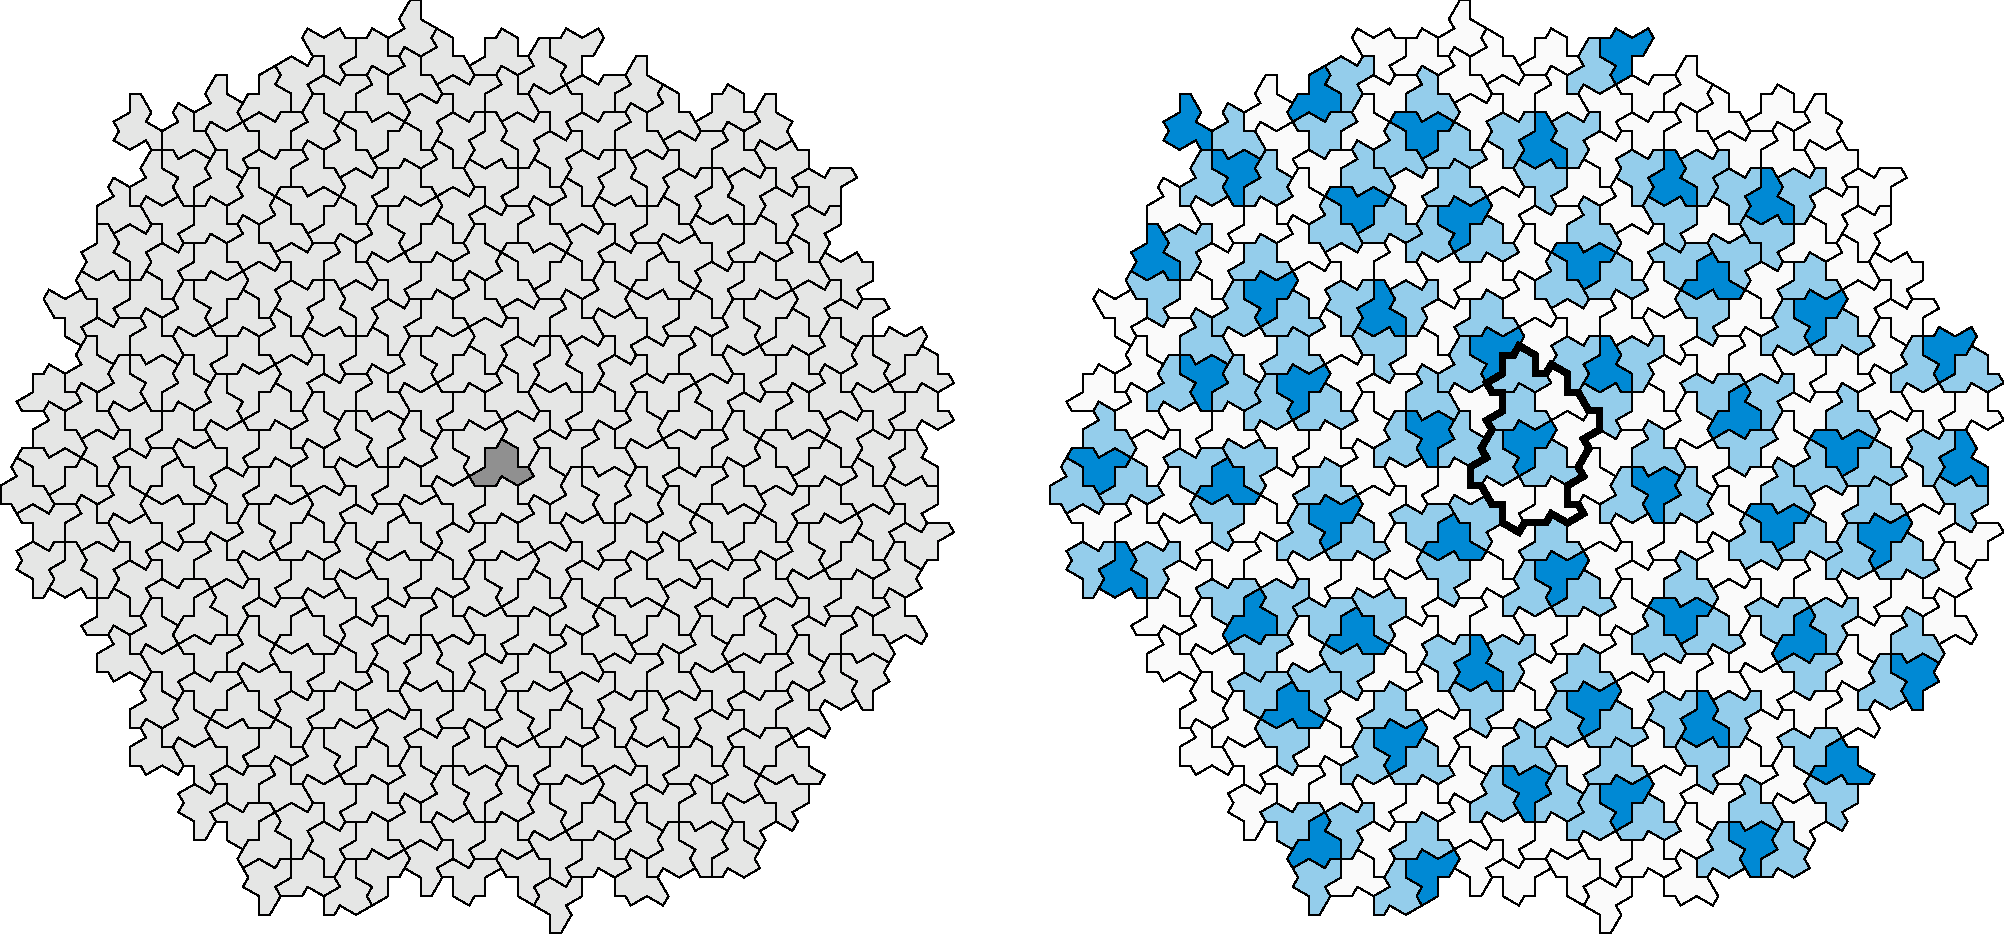
\includegraphics[width=\textwidth]{patch_alt.pdf}
\end{center}
\caption{\label{fig:patch10}A computer-generated $10$-patch of 392 hats
	(left), arranged in ten concentric rings around a central shaded hat.
	The tiles can be coloured (right), showing that the reflected 
	hats (dark blue) are sparsely distributed and each is surrounded by
	a congruent ``shell'' of three unreflected hats (light blue).
	A thickened outline shows the boundary of the maximal cluster
	of tiles that appears congruently around every reflected tile.}
\end{figure}

\fig{fig:patch10} (left) shows a computer-generated $10$-patch 
(i.e., ten concentric rings of tiles around a shaded central tile,
where each tile in a ring touches the ring it encloses in at least one 
point).  It was constructed by allowing Kaplan's software to work outward to
that radius, and then stopping it manually.
At first glance, it can be difficult to discern any
structure at all in this patch.  However, by colouring the tiles in different
ways, clear ``features'' begin to emerge.  Of course, we cannot infer any
conclusive properties of infinite tilings from a finite computed patch.
We must be particularly wary of tiles near the periphery of the patch,
where features may break down under the extra freedom afforded by
the proximity to empty space.  However, for a sufficiently large patch,
we might hope that tiles near the centre will be representative of 
configurations that arise in generic tilings.

\begin{figure}[htp!]
\begin{center}
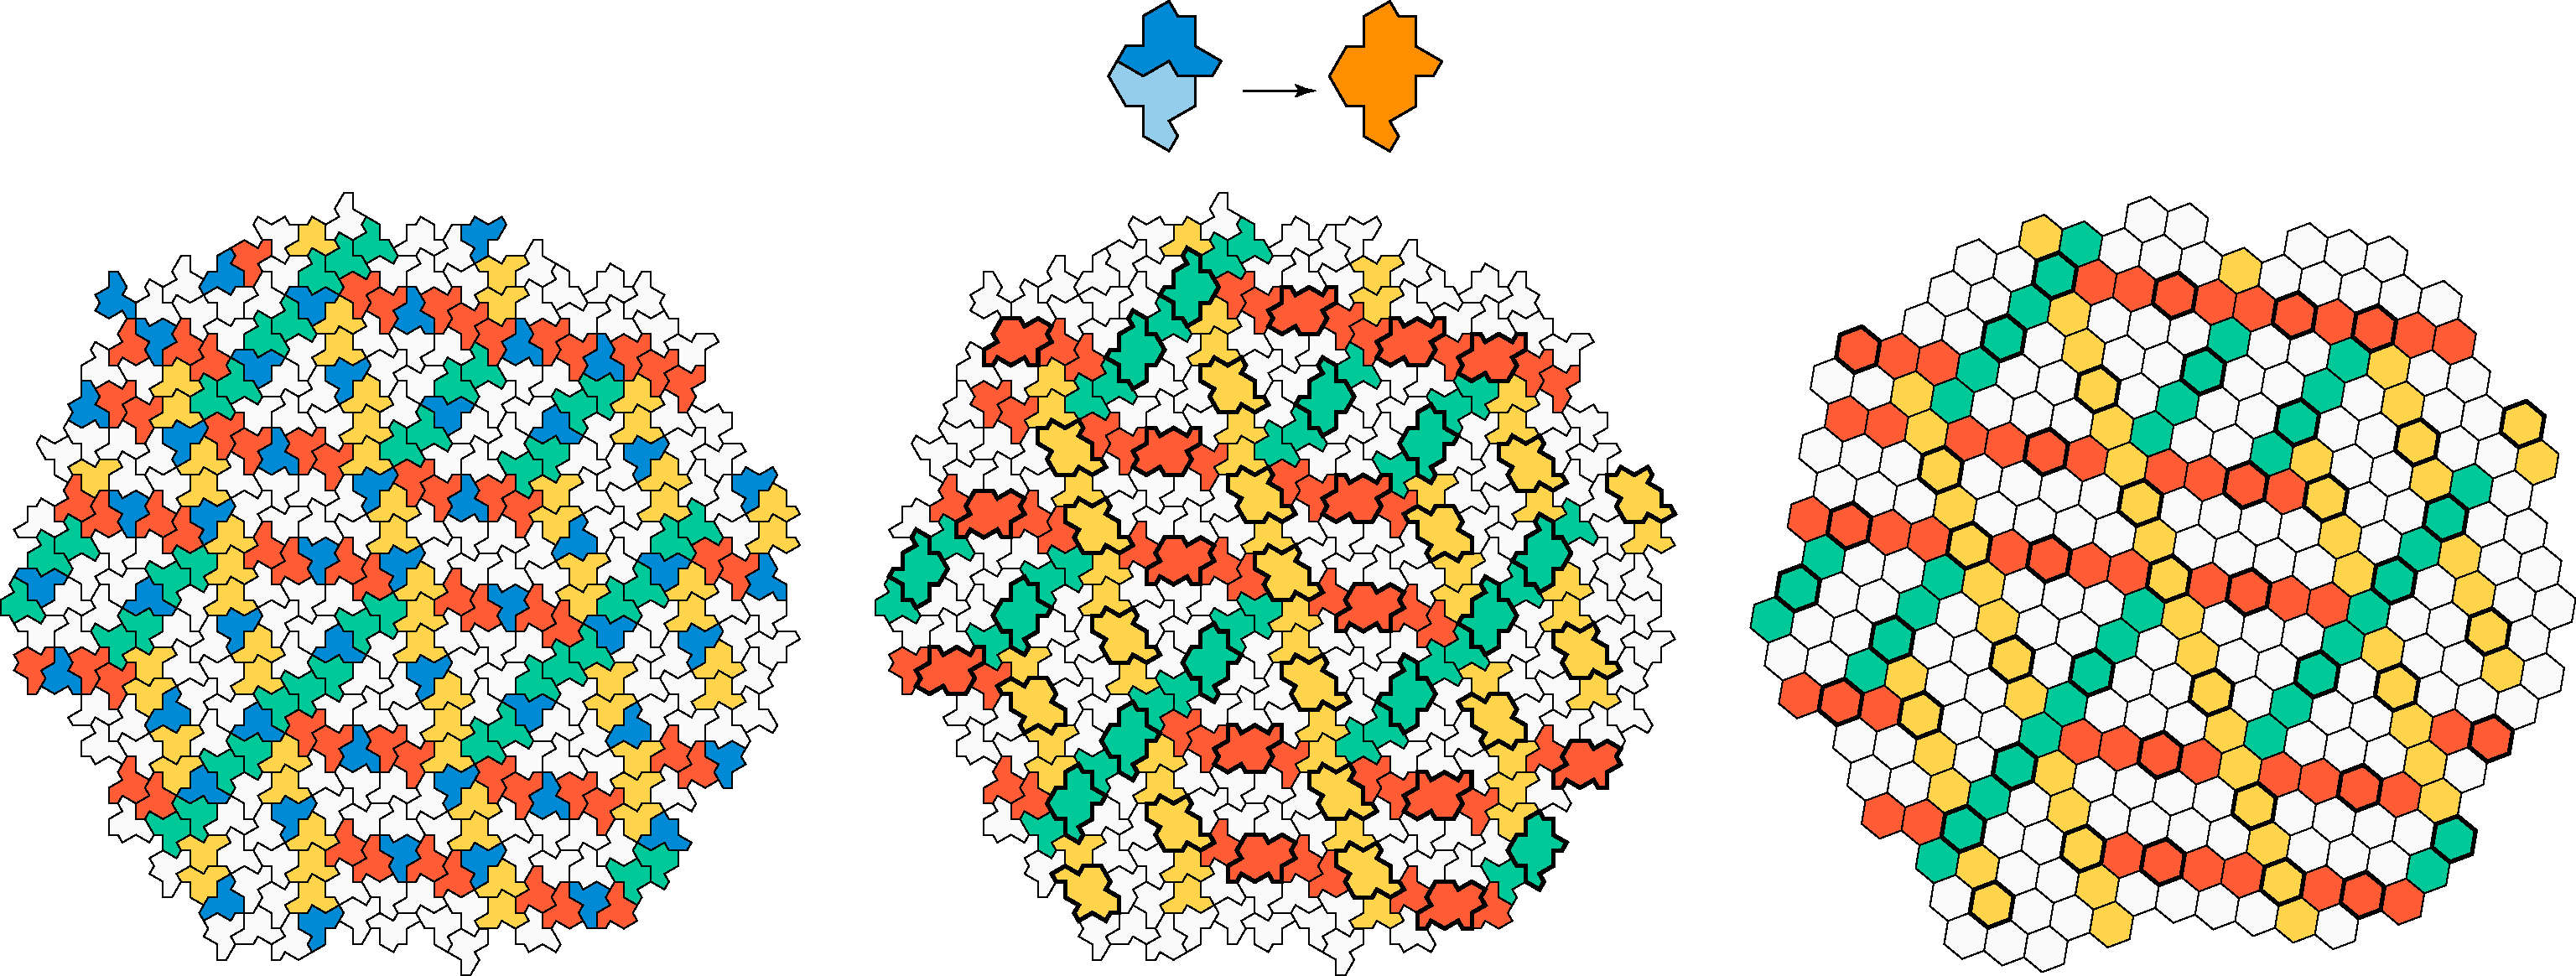
\includegraphics[width=\textwidth]{chains.pdf}
\end{center}
\caption{\label{fig:patch10col}
	Long chains of similarly oriented tiles pass through reflected tiles
	in six directions (left).  We can merge each reflected tile with one
	of its neighbours in its chain (centre), yielding a structure
	that can be placed into one-to-one correspondence with a patch of
	regular hexagons (right).}
\end{figure}

The most important colouring for the purposes of this article is the one shown
on the right in \fig{fig:patch10}.  A single hat is asymmetric, 
and so in any patch we can distinguish between ``unreflected'' and 
``reflected'' orientations of tiles.  In the patches we computed,
reflected tiles, shown in dark blue, are always
distributed sparsely and evenly within a field of unreflected tiles.
Furthermore, every reflected tile is contained within a congruent cluster
of nine tiles, where the other eight tiles in the cluster are unreflected.
One such cluster is outlined in bold in the illustration.  The interior of
the patch can be covered completely by overlapping copies of that cluster.
Within the cluster, we are particularly interested in the ``shell'' of 
three light blue tiles adjacent to each reflected tile.  Every reflected tile
resides in a congruent, non-overlapping copy of this shell.

We have also observed that unreflected tiles tend to form long
``chains'' of like orientation, occasionally interrupted by reflected
tiles.  The chains contained in the example patch are shown coloured
on the left in \fig{fig:patch10col}.  Because the hats are aligned
with the underlying kite grid, unreflected tiles come in six
orientations, all of which also appear as chain directions.  Chains
may end at reflected tiles or pass through them, but each reflected
tile is a hub for at least two, and at most five spokes.  
Long segments of these chains have boundaries with halfturn symmetry.
It is tempting to seek parallels between these chains and linear
features in other aperiodic tilings, such as Ammann bars~\cite[Section
10.6]{GS} and Conway worms~\cite[Section 10.5]{GS}.
Finally, we have noticed that these chains seem to impart a rough
hexagonal arrangement to the hats, which is particularly clear in the
triangular and parallelogram-shaped structures that are surrounded
by chains.  We have found that if we merge each reflected tile with its
immediate neighbour as shown in \fig{fig:patch10col} (centre), then the
tiles in any patch can be put into one-to-one correspondence with a 
patch of hexagons, as in \fig{fig:patch10col} (right).  The hexagonal grid
may provide a convenient domain in which to perform computations on the
combinatorial structure of tilings by hats.

\begin{figure}[htp!]
\begin{center}
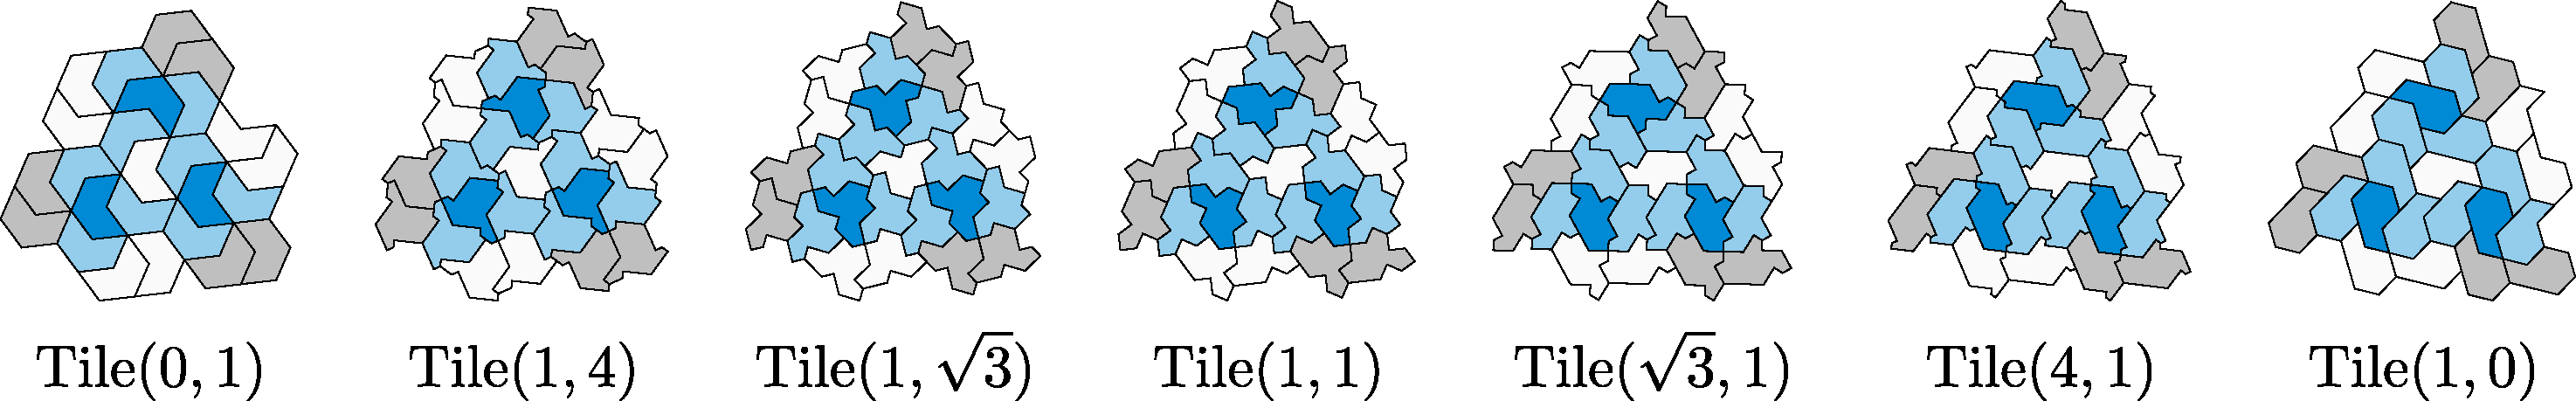
\includegraphics[width=\textwidth]{tile_ab.pdf}
\end{center}
\caption{\label{fig:tile_ab}The two edge lengths in the hat polykite
	can be manipulated independently, producing a continuum of shapes.
	A selection of those shapes is shown here, normalized for scale.
	$\mathrm{Tile}(0,1)$, $\mathrm{Tile}(1,1)$, and $\mathrm{Tile}(1,0)$ 
	admit periodic tilings; all others are aperiodic.}
\end{figure}

In the course of his explorations, the first author discovered a
\emph{second} polykite that did not seem to have a finite isohedral
number or a finite Heesch number, this one a union of ten kites.
The idea of identifying two einsteins back-to-back seemed too good to be 
true!  It was both a relief and a revelation when we determined that not
only were the hat and the $10$-kite related, they were in fact two
points from a continuum of shapes that all tile the plane the same
way.  The hat is derived from the $[3,4,6,4]$ grid, and therefore its edges
come in two lengths, which we can take to be $1$ and $\sqrt{3}$.  Furthermore,
these edges come in parallel pairs, allowing us to set the two lengths
independently to any non-negative values.  We use the notation 
$\mathrm{Tile}(a,b)$ with $a$ and $b$ not both zero to refer to the shape
produced when the length-$1$
and length-$\sqrt{3}$ edges are altered to have lengths $a$ and $b$,
respectively.  Note that $\mathrm{Tile}(a,b)$ is similar to
$\mathrm{Tile}(ka,kb)$ for any $k\neq 0$.  In \fig{fig:tile_ab} we show
a selection of shapes along this continuum, normalized for scale.
By this reckoning, the hat is $\mathrm{Tile}(1,\sqrt{3})$ and the 
$10$-kite is $\mathrm{Tile}(\sqrt{3},1)$.
We have also created an animation showing a continuous evolution
of $\mathrm{Tile}(a,1-a)$ as $a$ moves from $0$ to $1$ and back---see
\href{https://youtu.be/W-ECvtIA-5A}{\nolinkurl{youtu.be/W-ECvtIA-5A}}.
The tetriamond $\mathrm{Tile}(0,1)$, the octiamond $\mathrm{Tile}(1,0)$,
and the equilateral $\mathrm{Tile}(1,1)$ admit simple periodic tilings;
in \secref{sec:family}, we will show that all other shapes in this continuum
are aperiodic monotiles with combinatorially equivalent tilings.
In \secref{sec:coupling}, $\mathrm{Tile}(0,1)$ and $\mathrm{Tile}(1,0)$ 
will play a crucial role in establishing that the hat is aperiodic.
Inspired by cut-and-project methods~\cite{deBruijn1,deBruijn2}, we are also left
wondering
whether it would be productive to construct a closed path in four or
six dimensions, which projects down to this family of tiles from a suitable
set of directions.

\begin{figure}[htp!]
\begin{center}
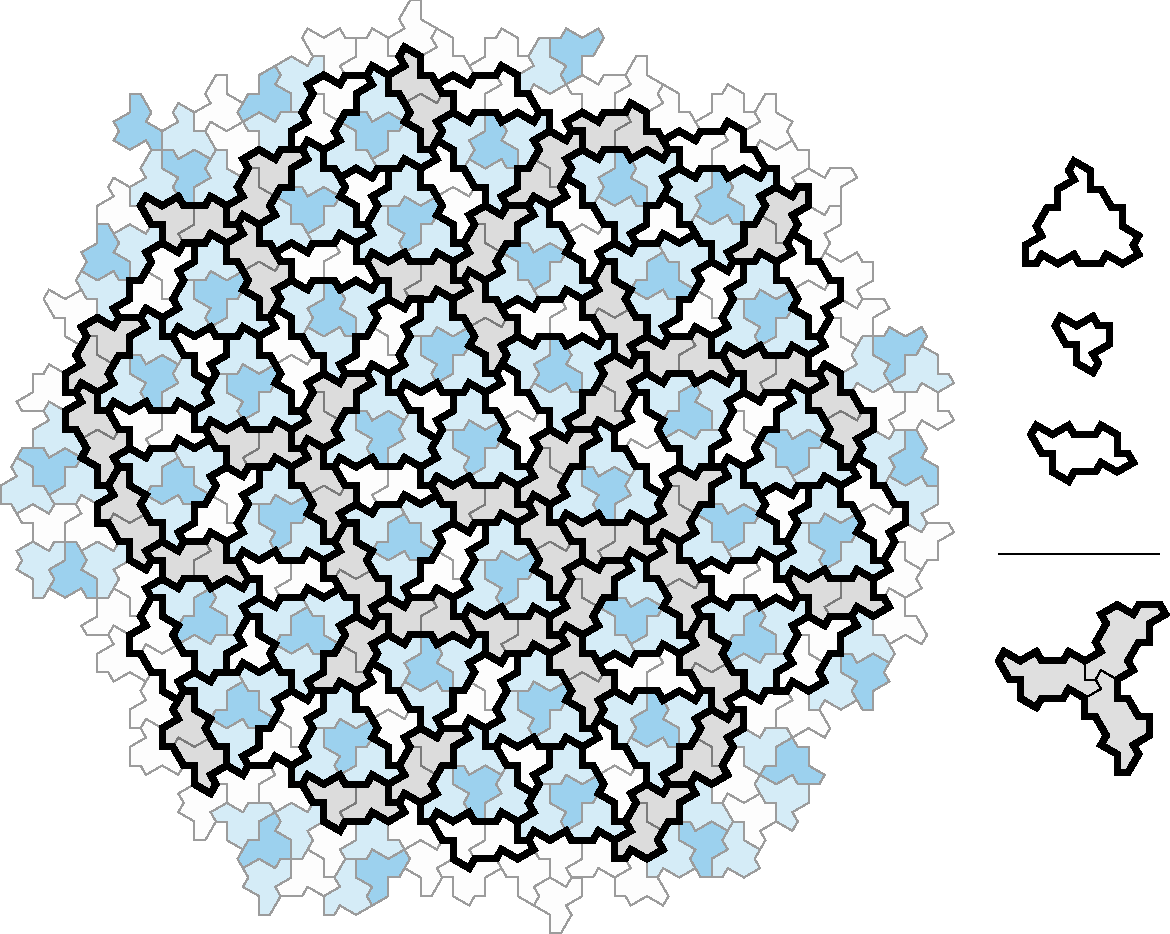
\includegraphics[height=2.75in]{patch_10_clusters_b.pdf}
\end{center}
\caption{\label{fig:patch10clu}A grouping of tiles into clusters in the
	example patch.  In addition to four-tile clusters consisting of a 
	reflected hat and its three-hat shell, we identify clusters consisting
	of a single tile, and parallelogram-shaped clusters consisting of
	pairs of tiles. The parallelograms come in two varieties: one 
	separates two nearby shells, and the other joins up with two rotated
	copies to make a three-armed propeller shape called a \textit{fylfot}.
	An isolated fylfot is shown shaded in grey in the lower right.}\end{figure}

Given the colouring in \fig{fig:patch10col} showing non-overlapping
clusters of reflected tiles and their shells,
it is natural to wonder whether the remaining unaffiliated tiles in the
patch reliably 
form clusters of other kinds.  \fig{fig:patch10clu} illustrates that we can
account for all remaining tiles using two additional cluster types (shown
separately on the right).  First,
where three shells meet they enclose a single isolated tile, which must be
accepted as a cluster of size one.  Then the remaining tiles group into
congruent clusters of size two, which are roughly parallelogram-shaped.
These appear in two varieties, depending on the local arrangement of
clusters around them.  In the first case, coloured white in the drawing,
the parallelogram is adjacent to
two shells along its long edges.  In the second case, coloured grey,
one end of the 
parallelogram is plugged into a local centre of threefold rotation, joining
six hats into a three-armed propeller shape called a \textit{fylfot}.
A fylfot is shown in isolation on the bottom right of \fig{fig:patch10clu}.

These clusters are the starting point for the definition of a
substitution system, one that can be iterated to produce a patch
of hats of arbitrary size.  Interestingly, the substitution rules
do not apply to the hats directly.  Instead, we derive new \textit{metatiles}
from the clusters, and build a substitution system based on the
metatiles. The underlying hats are simply brought along for the
ride.

\begin{figure}[htp!]
\begin{center}
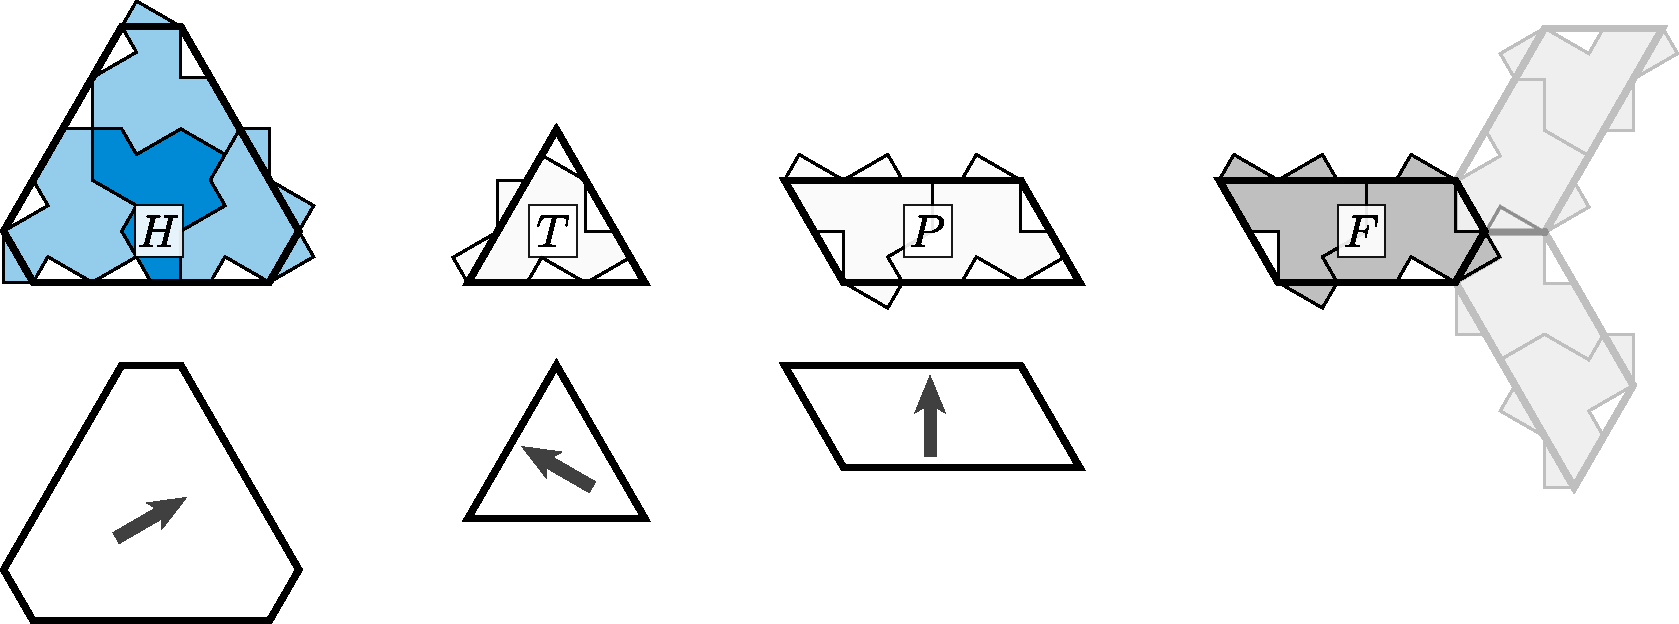
\includegraphics[width=0.75\textwidth]{simplified_outlines.pdf}
\end{center}
\caption{\label{fig:simp_outlines}The $H$, $T$, $P$, and $F$ metatiles (top),
	constructed by simplifying the boundaries of clusters of hats.
	We mark the $H$, $T$, and $P$ metatiles with arrows when needed (bottom),
	to distinguish between otherwise symmetric orientations.}
\end{figure}

\fig{fig:simp_outlines} shows the shapes of the metatiles.  Each
one is constructed by simplifying the boundary of one of the clusters
of hats in \fig{fig:patch10clu}.  In order to ensure that the metatiles
do not overlap, we must distinguish between the two varieties of two-hat
parallelograms discussed above.  Specifically, we remove a triangular
notch from the parallelogram associated with each blade of a fylfot.  Thus
the three clusters yield four metatiles: an irregular hexagon ($H$), 
an equilateral triangle ($T$), a parallelogram ($P$), and a pentagonal
fylfot blade ($F$).
The original clusters can now
be seen as endowing the metatiles with matching conditions
along their edges; these matching conditions will be formalized in
\secref{sec:clusters}.

The $H$, $T$, and $P$ metatiles have rotational symmetries.
In the bottom row of \fig{fig:simp_outlines}, we mark tiles
with arrows showing their intended orientations.  In each case, the
arrow points to the (unique) side of the metatile from which two adjacent
kites protrude.  The arrows suffice to distinguish symmetric rotations
and our construction will not use reflections. (We will not need these
arrows in later sections, as metatile orientations will be implied by 
labels on their edges.)

\begin{figure}[htp!]
\begin{center}
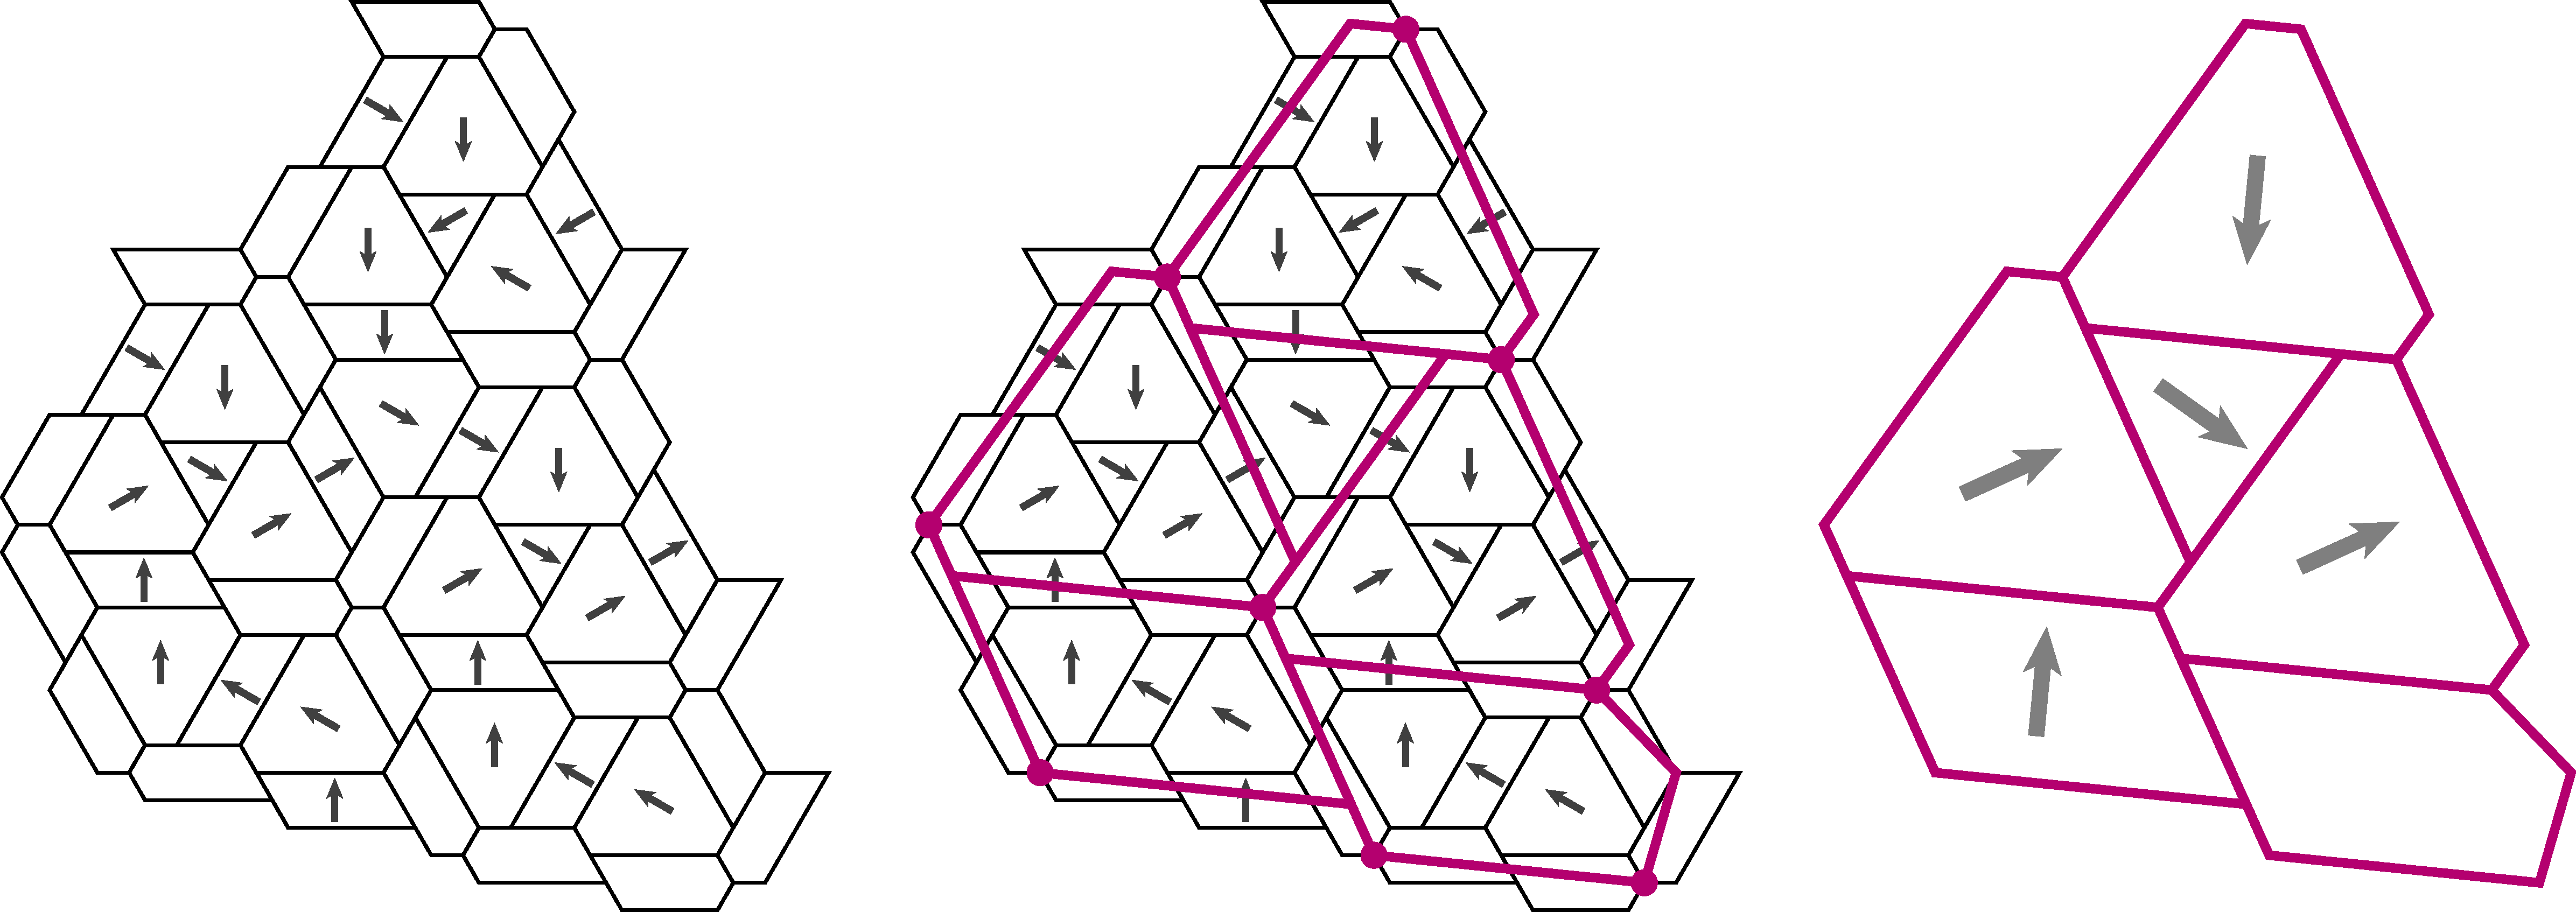
\includegraphics[width=0.95\textwidth]{supertiles.pdf}
\end{center}
\caption{\label{fig:supertiles}The construction of a family of 
	supertiles from a patch of metatiles.  The patch of metatiles on
	the left can be used to locate key vertices of the supertiles,
	marked with red dots in the central diagram.  Those dots, 
	together with constraints on angles, fully determine the shapes
	of the supertiles, which are not merely scaled-up copies of their
	progenitors.  On the right, the supertiles are marked with
	arrows indicating their orientations.}
\end{figure}

We can now define a family of supertiles that are analogous to the
metatiles, following the procedure illustrated in 
\fig{fig:supertiles}.  We first assemble the patch of oriented metatiles
shown on the left.  It can easily be checked that the elided
hat polykites borne by these tiles fit together with no gaps and no
overlaps.  This patch is large enough to pick out one
or more copies of 
each supertile, drawn in red in the central diagram.
The supertile shapes are fully determined by two constraints:
the red dots coincide with the centres of fylfots, and all interior angles
of the hexagonal outlines are $120^\circ$.  The diagram on the right 
shows the supercluster outlines in isolation, with their inherited
orientation markings.  Here, each arrow points to the unique supertile
edge that passes through an outward-pointing $P$ tile from the previous
generation.

\begin{figure}[ht!]
\begin{center}
\includegraphics[width=\textwidth]{hexclusters.pdf}
\end{center}
\caption{\label{fig:hexclusters}The first four iterations of the 
	$H$ metatile and its supertiles.  At each level, tiles partially
	overlap the boundary of their supertile.  Overlaps are acceptable
	here, because the supertile will be met by neighbouring supertiles
	with the same configuration of smaller tiles on its boundary.}
\end{figure}


\begin{figure}[ht!]
\begin{center}
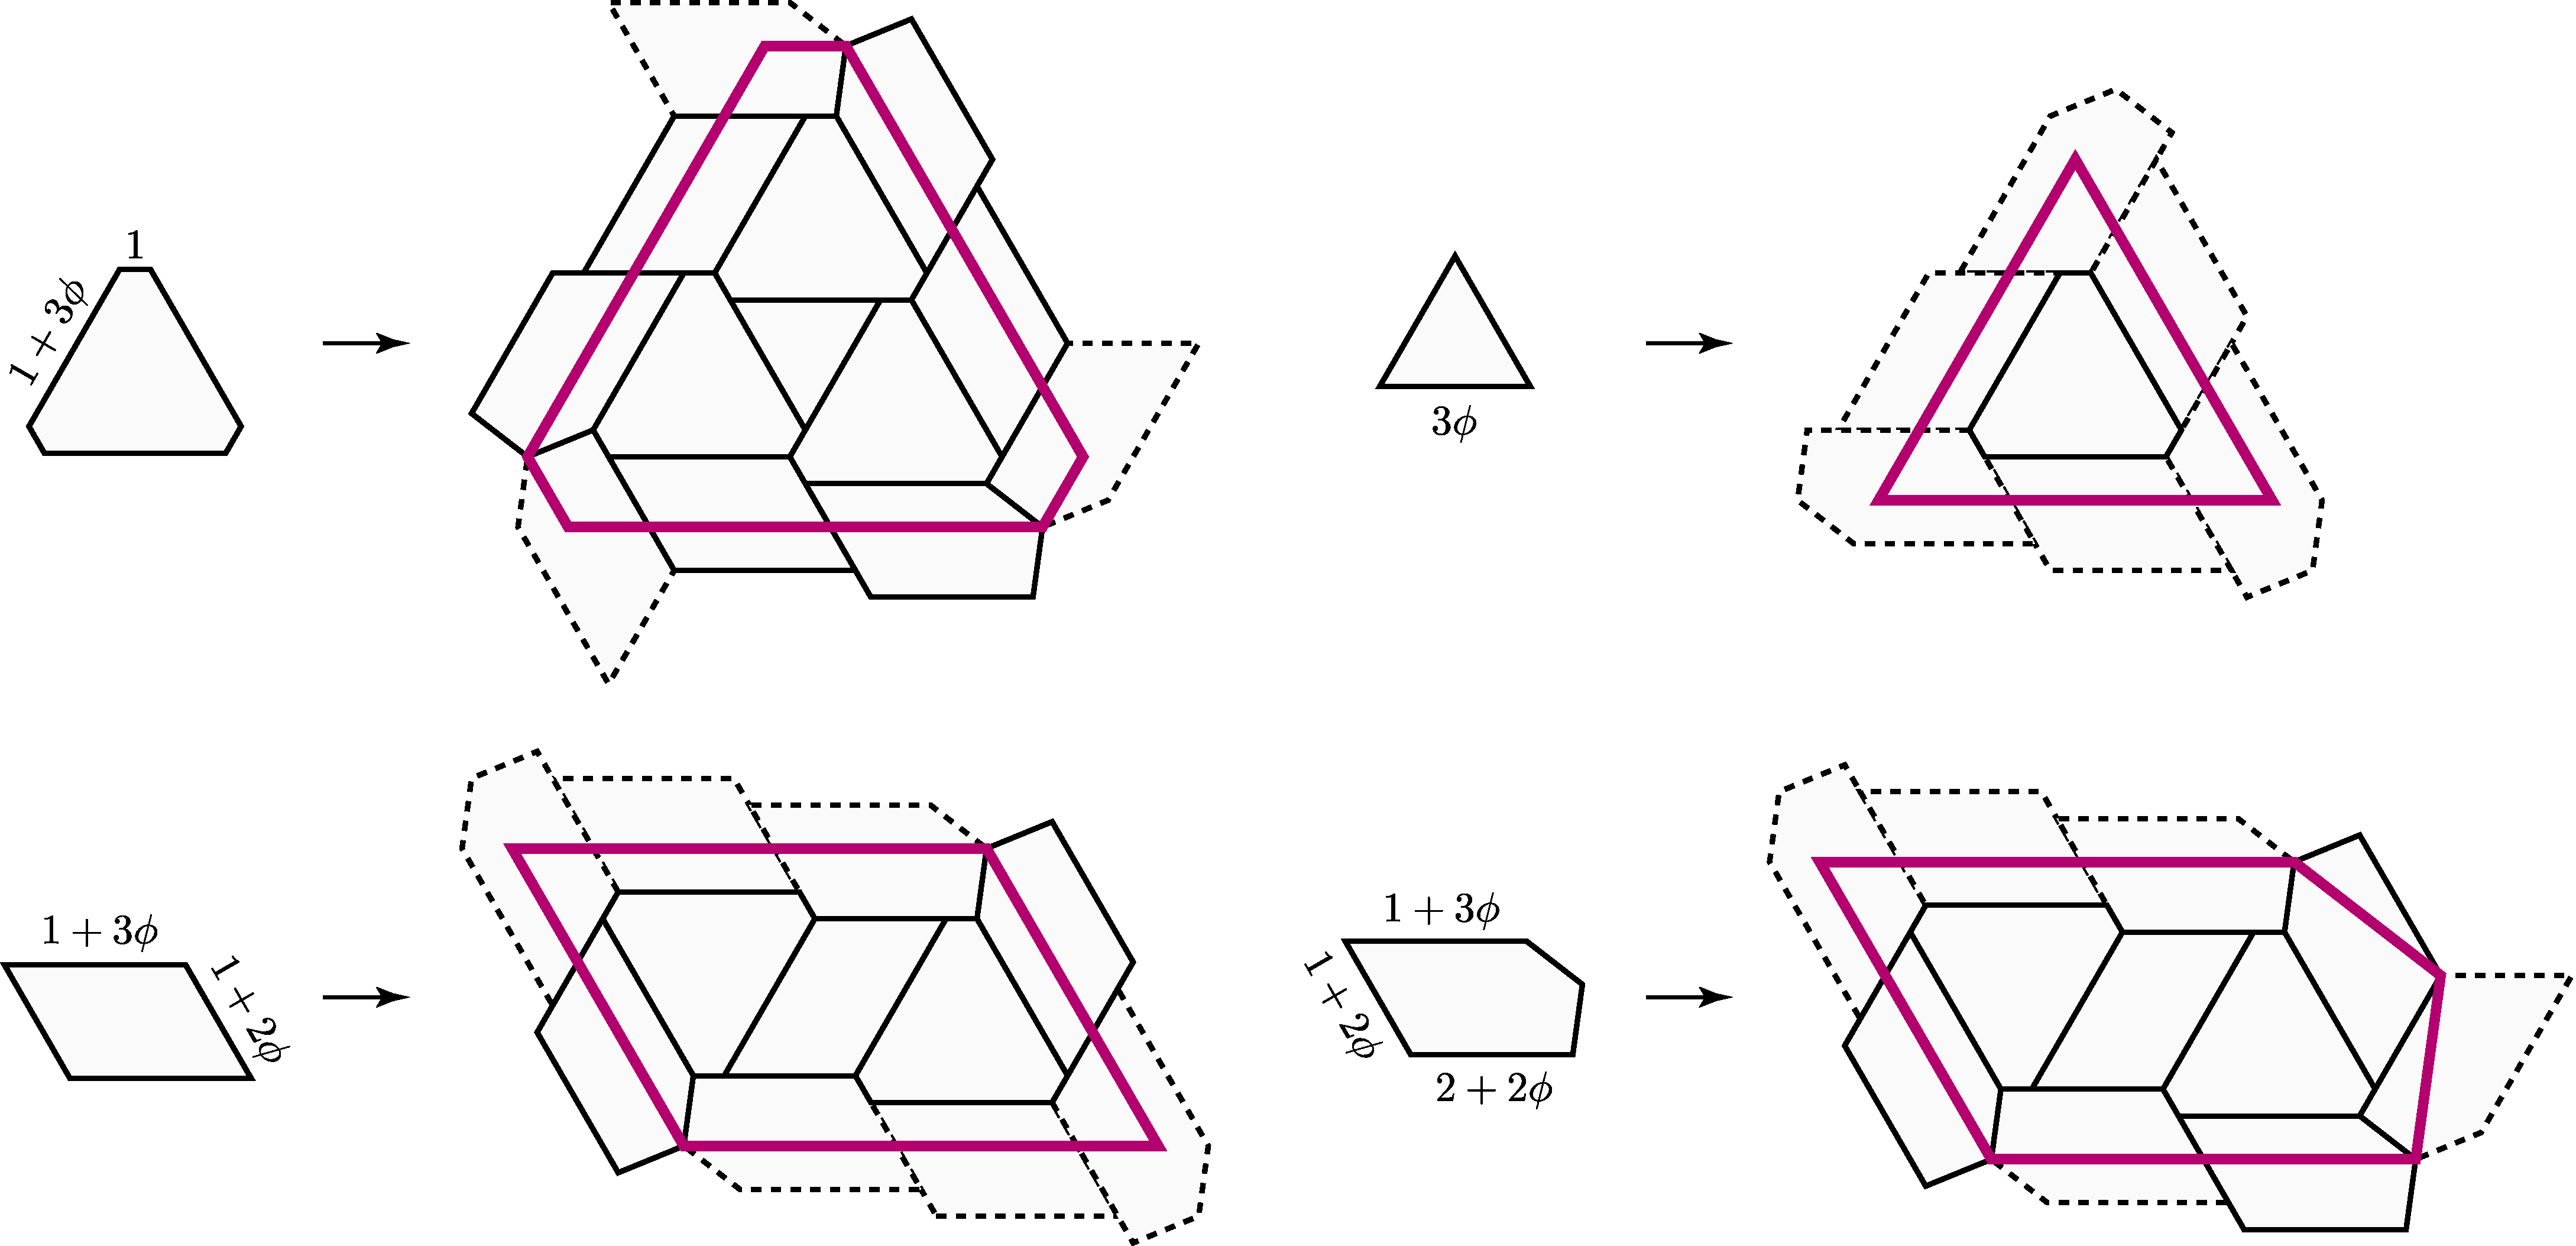
\includegraphics[width=\textwidth]{perfect_sub.pdf}
\end{center}
\caption{\label{fig:perfect}A substitution system based on converged
	tile shapes.  Scaling the tiles so that the the short edges of the $H$
	tile have unit length, all tile edges except the two adjacent to fylfot 
	centres
	have lengths in $\mathbb{Z}[\phi]$, where $\phi$ is the golden ratio.
	In each substitution rule, tiles shown with dashed boundaries can be 
	omitted, leading to patches in which there are no duplicate tiles
	contributed by supertiles sharing an edge.}
\end{figure}

At first glance, these supertiles appear to be scaled-up copies
of the metatiles.  If that were so, we could perhaps proceed to
define a typical substitution tiling, where each scaled-up supertile is
associated with a set of rigidly transformed tiles.  However, with
the obvious exception of the $T$, none of the 
supertiles is truly similar to its corresponding metatile.
Despite that discrepancy, the supertiles are fully
compatible with the construction in \fig{fig:supertiles}---they
can be arranged in the same configuration shown on the left, and used as
a scaffolding for deriving outlines of super-supertiles (implicitly
yielding a much larger patch of hats along the way).  Indeed, the construction
can be iterated any number of times, with slightly different outlines in
every generation.  We are not aware of other substitution systems that
use rules like these, where successive generations are combinatorially
but not geometrically compatible.
To see this construction in action, please try our interactive
browser-based visualization tool at
\href{https://cs.uwaterloo.ca/~csk/hat/}{\nolinkurl{cs.uwaterloo.ca/~csk/hat/}}.

We know from \fig{fig:simp_outlines} that each of the four metatiles
can be associated with a cluster of hats.  The construction in
\fig{fig:supertiles} can then be iterated any number of times to form
ever-larger patches of metatiles, and hence of hats.  We can, for 
example, consider the $H$ supertiles formed through this process of
iteration, and the patch of hats each one contains.  These patches form
a sequence that grows in radius without bound, each patch a subset of
its successor.  The Extension Theorem~\cite[Section 3.8]{GS} allows
us to continue this iteration process ``to infinity'', yielding the
following result.

\begin{theorem}
\label{thm:subst_tiling}
	The hat polykite admits tilings of the plane.
\end{theorem}

Of course, this theorem is not sufficient to establish aperiodicity
on its own---we must also show that the hat does not also admit
periodic tilings.  In \secref{sec:subst} we revisit this
substitution process, tracking matching conditions on supertile edges
after every step.  There we show that \textit{all} tilings by the 
hat necessarily obey the substitution rules given here
(Theorem~\ref{thm:subst}).  The construction in that section also
incidentally leads to a more detailed proof that the hat tiles the plane.

The shapes of each generation of supertiles are different from those
of the generation before it.  However, by normalizing the tiles for
size, we have computed that they quickly converge on a fixed point, a 
set of tiles that truly do yield scaled copies of themselves under the
construction in \fig{fig:supertiles}.  These converged tile
shapes are particularly interesting because they can be used to define a 
geometric substitution system that operates via inflation and replacement.
The converged tiles, together with
their substitution rules, are shown in \fig{fig:perfect}.
By virtue of its connection to the original metatiles in
\fig{fig:simp_outlines}, we know that this substitution tiling is aperiodic
when the tiles are endowed with suitable matching conditions on their
edges.  We can also use this system as an alternative means of constructing 
patches of hats.  We cannot simply associate a cluster of hats rigidly with
each converged tile, but a patch of converged tiles is combinatorially
equivalent to a corresponding patch of metatiles, which are
equipped with hats.

If we rescale the converged tiles so that the short $H$ edges
have unit length, then all tile edges except the two $F$ edges adjacent to
a fylfot centre will have lengths in $\mathbb{Z}[\phi]$, where $\phi$ is the
golden ratio.  Furthermore, this substitution system has an inflation factor
of $\phi^2$.  The factor of $\phi^2$ can also be derived algebraically, 
through an eigenvalue computation on the substitution matrix corresponding to
the system presented in
this section.

\begin{figure}[ht!]
\begin{center}
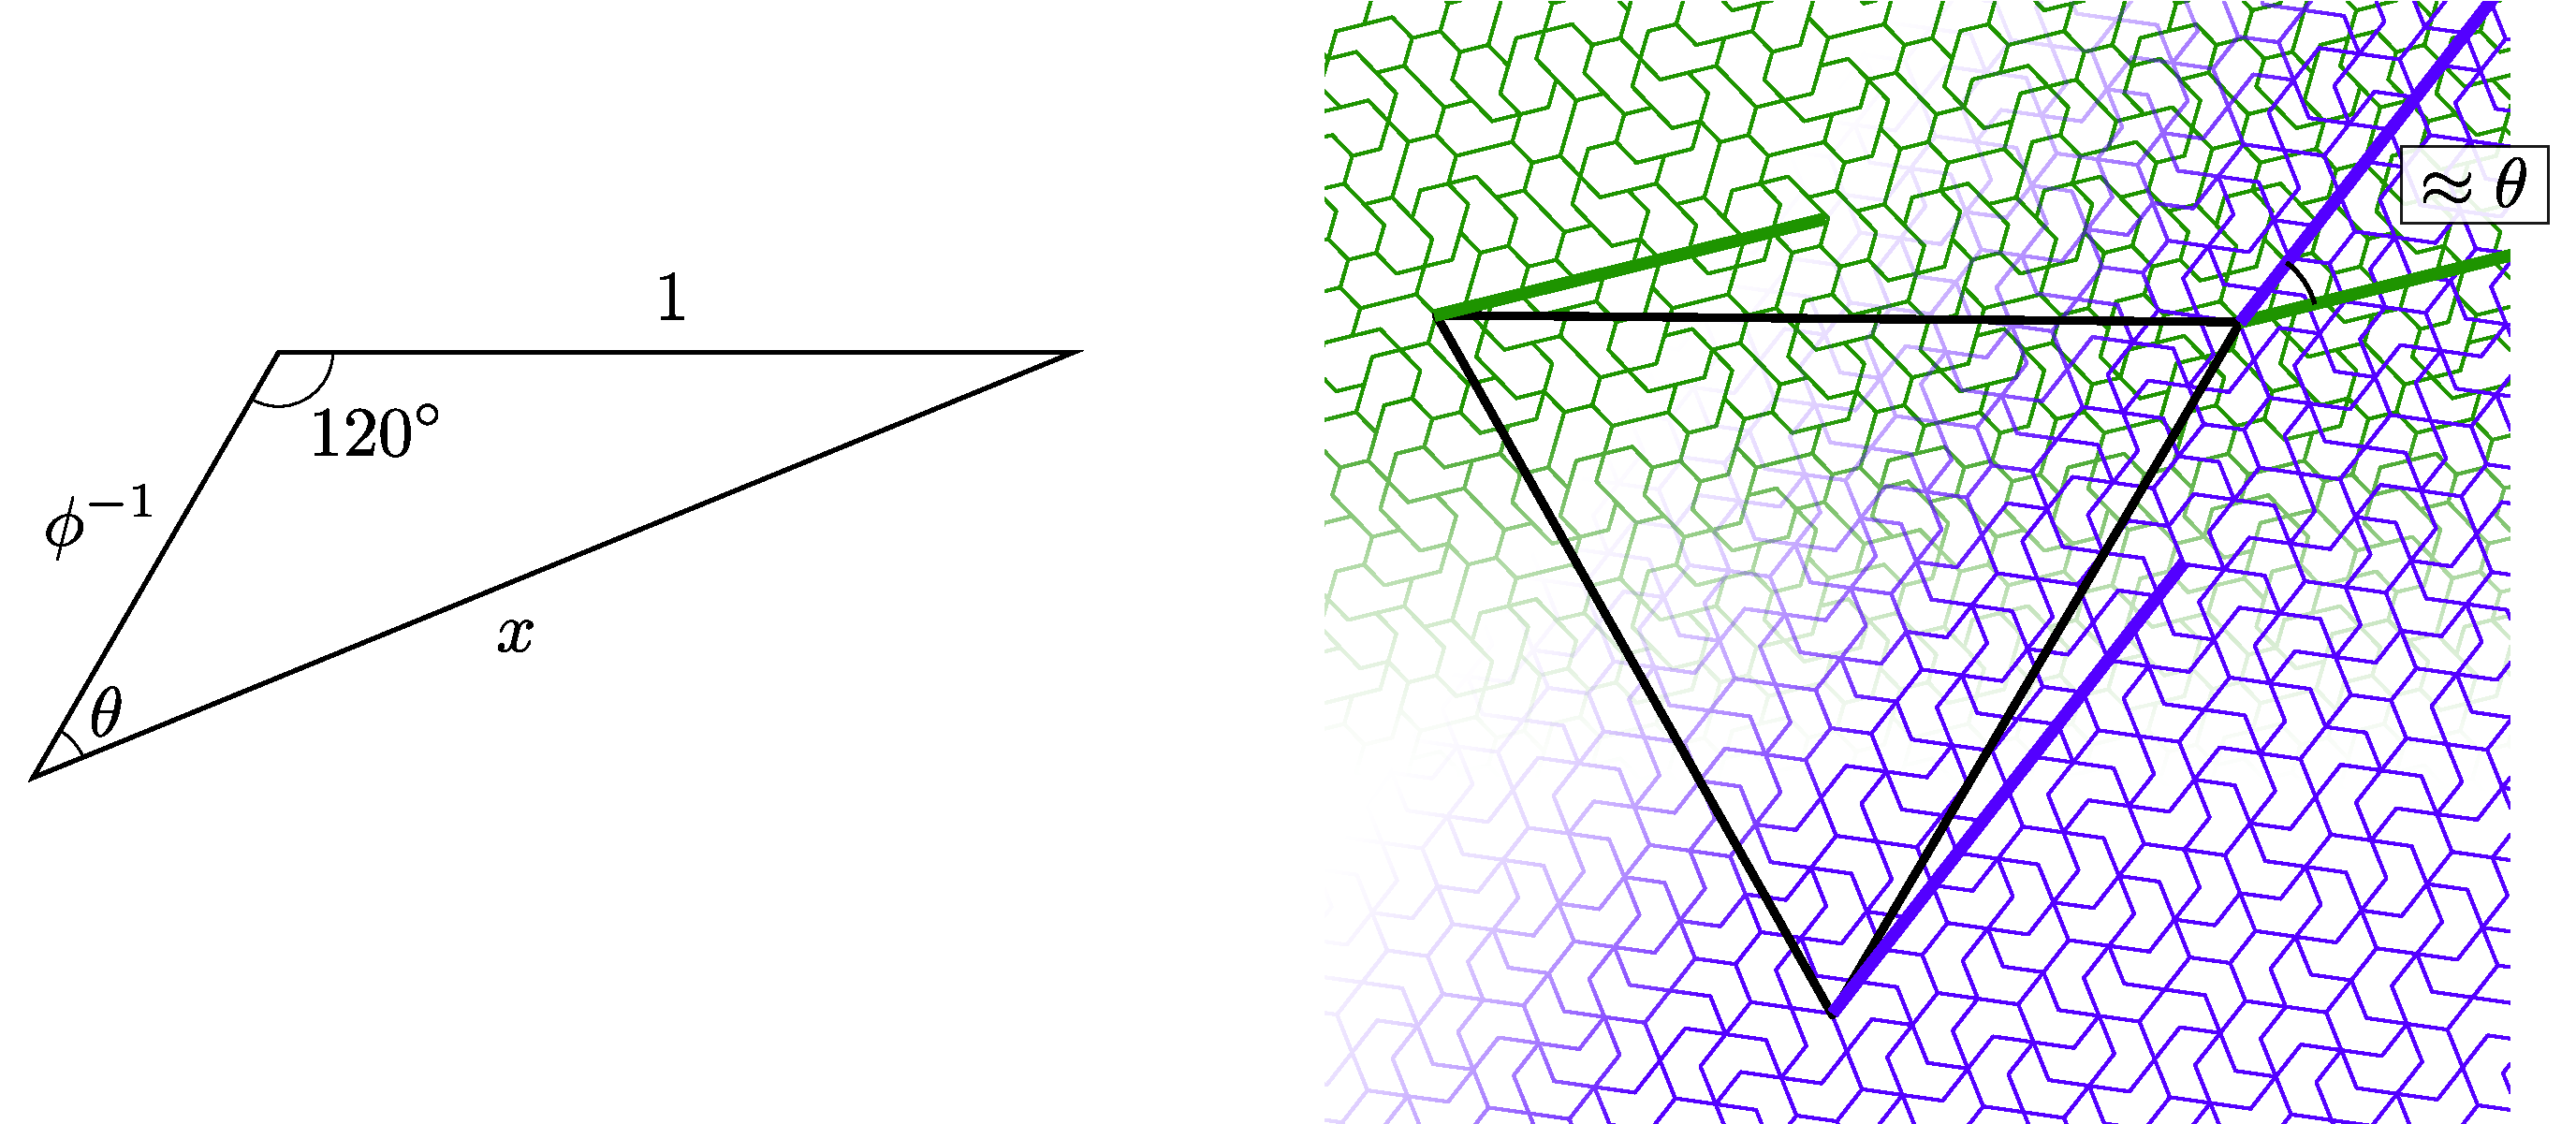
\includegraphics[width=0.75\textwidth]{arctan2.pdf}
\end{center}
\caption{\label{fig:arctan}
	A demonstration of how the golden ratio $\phi$ might arise in
	the context of tilings by hats.  The triangle on the left has
	an angle of $120^\circ$ between sides of lengths $1$ and $\phi^{-1}$;
	from trigonometric identities we can compute that $x=\sqrt{2}$ and
	$\theta=\tan^{-1}\sqrt{3/5}$.  On the right we show portions
	of tilings by $\mathrm{Tile}(1,0)$ (green) and $\mathrm{Tile}(0,\sqrt{2})$
	(blue), registered to the same centres of local threefold rotation.
	The angle between the edges of the triangle tilings underlying these
	two polyiamond tilings is approximately $\theta$, and we believe this
	approximation converges as we register larger patches of the two
	tilings.}
\end{figure}

At first blush, it may be surprising to see $\phi$ arise
in a tiling closely associated with the Laves tiling $[3.4.6.4]$; it
appears more naturally in contexts such as Penrose tilings, which feature
angles derived from the regular pentagon.
The involvement of $\phi$ appears to be closely related to the
appearance of~$\sqrt{2}$ in the argument of \secref{sec:coupling};
that number is also not expected on the regular triangular tiling or
related contexts (where distances are the square roots of integers
that can be expressed by the quadratic form $x^2+xy+y^2$, so expected
square roots are of $3$ and primes of the form $6k+1$).  However, $1 +
\phi^{-1} + \phi^{-2} = 2$, from which it follows that a triangle with a
$120^\circ$~angle between sides of lengths $1$ and~$\phi^{-1}$ has
a third side of length~$\sqrt{2}$ (\fig{fig:arctan}, left).  And indeed,
by aligning corresponding tiles of tilings using
$\mathrm{Tile}(1,0)$ and $\mathrm{Tile}(0,\sqrt{2})$,
it appears that there is an angle
$\tan^{-1}\sqrt{3/5}$, which is one of the angles of the triangle with
sides $1$, $\phi^{-1}$, and~$\sqrt{2}$, between the edges of the
regular triangular tilings underlying $\mathrm{Tile}(1,0)$ and
$\mathrm{Tile}(0,\sqrt{2})$ (\fig{fig:arctan}, right).

The arrangement of three $H$ tiles and a $T$ tile inside of an $H$ 
supertile mimics the arrangement of a reflected hat and its three
unreflected neighbours in a single $H$ metatile.  We are naturally
led to wonder whether the clusters of hats that make up the metatiles
are primordial, or whether they are preceded by a set of ``subclusters''
that launch the substitution process one step earlier.
A possible form for such subclusters is shown in Figure~\ref{fig:subclusters}.
The labels on the edges denote matching conditions that will be explained
in detail in \secref{sec:clusters}.
Note that subclusters $P_0$ and~$F_0$
have zero area; their boundaries are shown split into multiple
parts to clarify the sequence of edges (in the case of~$F_0$, some of
those edges intersect others); note also that the $X^+$ and $X^-$
edges from Figure~\ref{fig:tileaclusters} have length zero in the
subclusters and are not shown in the diagram.  Defining what exactly
it means to partition a tiling into subclusters following matching
rules, when some subclusters have area zero and some edges have length
zero but must still adjoin in the correct orientations, seems 
more awkward than the corresponding argument
based on metatiles, so we do not pursue the subclusters further.

\begin{figure}[htp!]
\begin{center}
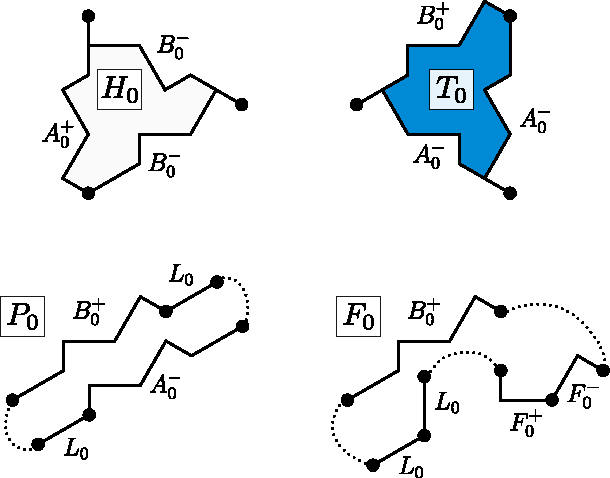
\includegraphics[width=3in]{subclusters.pdf}
\end{center}
\caption{\label{fig:subclusters}
	Four subclusters that may be thought of as preceding the clusters making
	up the metatiles in \fig{fig:simp_outlines}.  Edges are marked with
	the labels that will be used in \secref{sec:clusters}.  The
	$P_0$ and $F_0$ subclusters have zero area; dotted lines indicate 
	vertices that should be regarded as coincident.}
\end{figure}


\begin{figure}[htp!]
\begin{center}
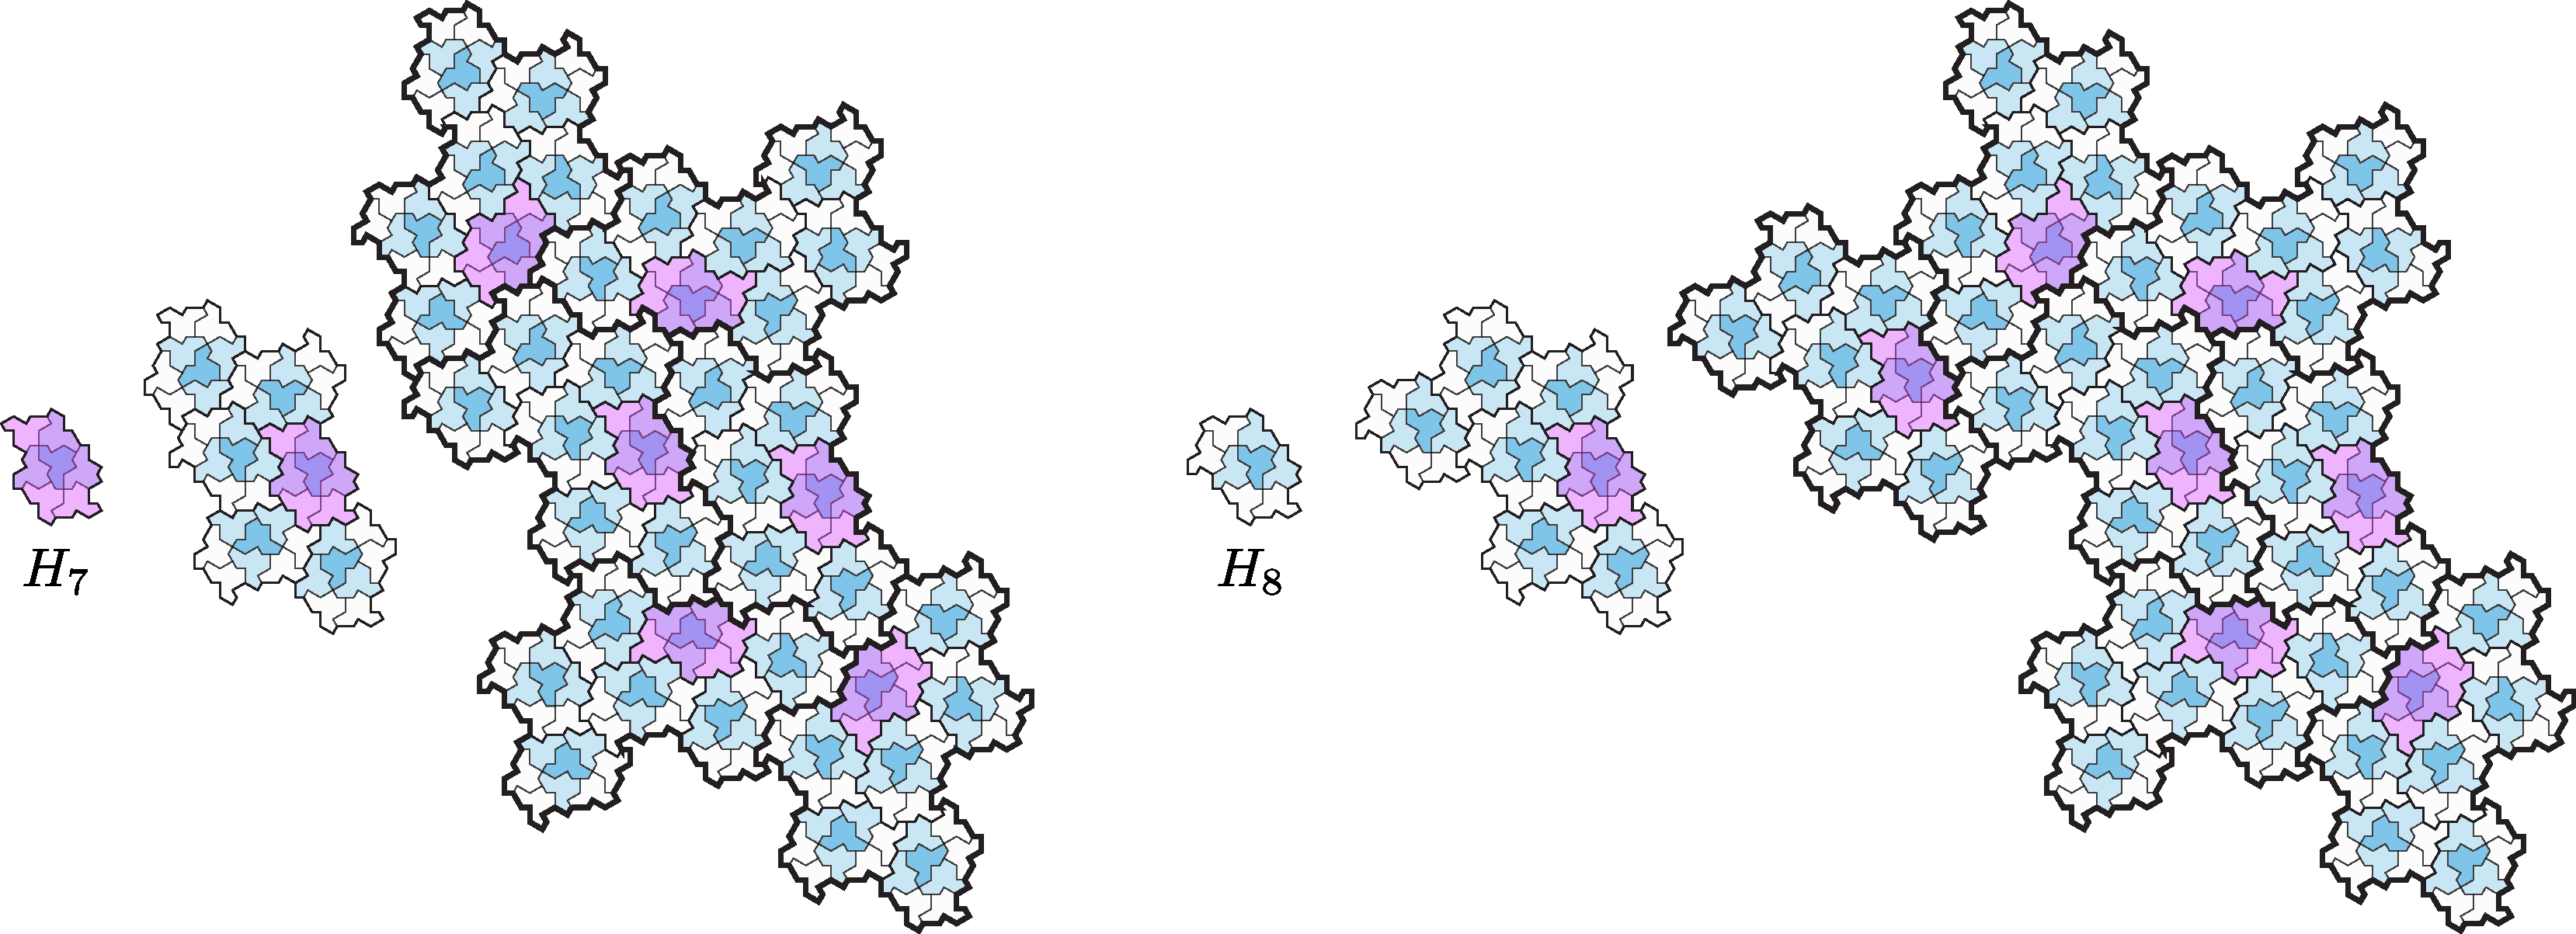
\includegraphics[width=\textwidth]{alt_subst.pdf}
\end{center}
\caption{\label{fig:alt_subst}An alternative substitution system that
	yields the same tiling by hats as the system presented earlier.
	Here there are clusters $H_7$ and $H_8$, made up of seven and eight
	hats, respectively.  Each one can be iteratively replaced by a 
	supercluster made up of copies of $H_7$ and $H_8$.}
\end{figure}

Finally, in \fig{fig:alt_subst} we  exhibit a second substitution system
in which hats are 
grouped into only two clusters instead of the four shown in 
\fig{fig:simp_outlines}.  The cluster $H_7$ comprises seven hats:
a reflected hat, its three-hat shell, and three additional neighbours. 
The cluster $H_8$ contains all of $H_7$ plus one additional neighbour.
As illustrated in the figure, $H_7$ and $H_8$ can be replaced by 
superclusters, each containing a single $H_7$ and five or six copies of
$H_8$. This 
process can then be iterated to produce a patch of hats of any size.
This substitution system is attractive for its minimality, though we 
believe it would be more cumbersome for proving aperiodicity.
Although the tilings themselves are MLD (mutually locally
derivable)~\cite{BaakeMLD}
with those by the $H$, $T$, $P$, and $F$ metatiles presented earlier,
deriving those metatiles from the $H_7$ and~$H_8$ clusters requires
considering a radius larger than a single cluster.
$H_7$ is always equivalent to the union of an
$H$ tile, a $T$ tile, and an $F$ tile, but $H_8$  corresponds
to three different combinations of $H$, $P$, and $F$.  Alternatively,
to establish an MLD
system, we could define three congruent but inequivalent copies
of $H_8$.

\begin{figure}[ht!]
\begin{center}
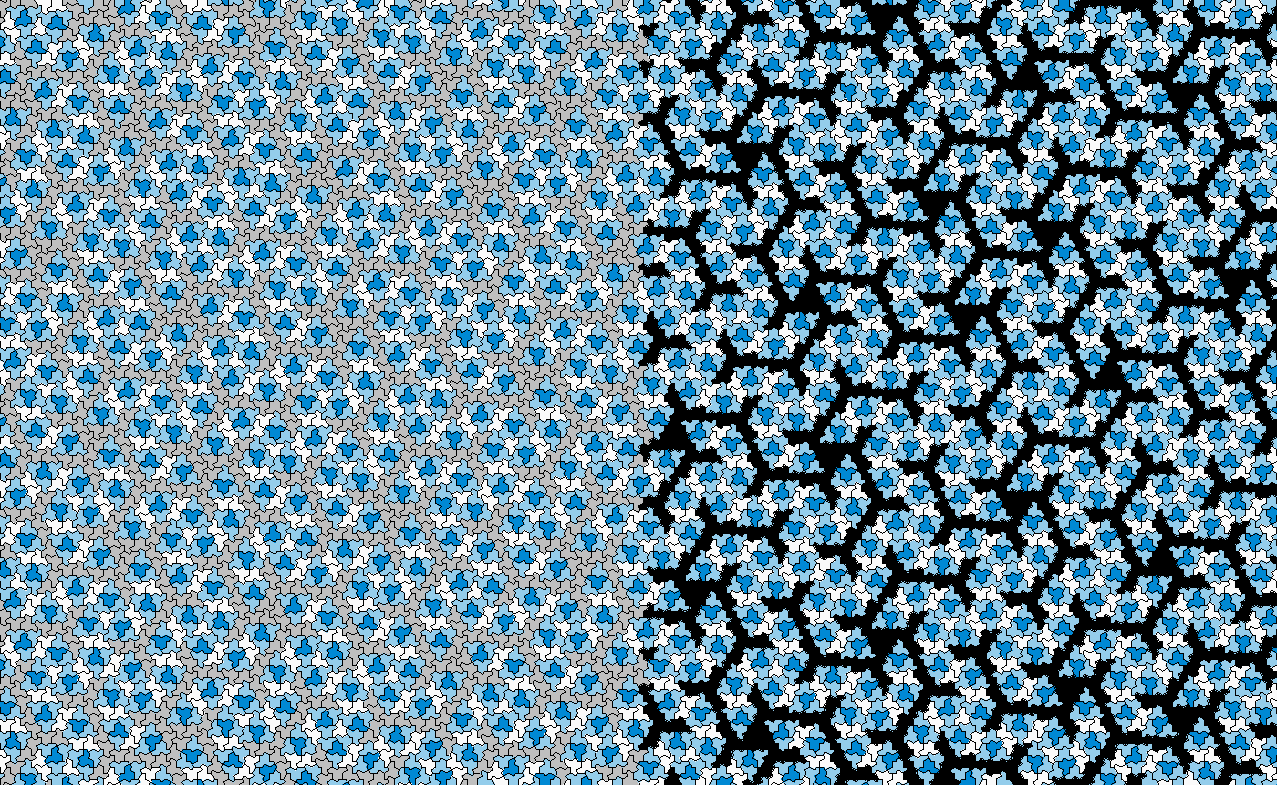
\includegraphics[width=\textwidth]{gargantuan.pdf}
\end{center}
\caption{\label{fig:gargantuan}An excerpt from a very large patch generated
	using the substitution system presented in this section.  In the right
	half of the drawing, hats belonging to $F$ metatiles are coloured black,
	to highlight the interlocking tree structures formed by the fylfots
	and the other metatiles.}
\end{figure}

The ideas presented in this section are sufficient to show that the
hat does in fact tile the plane.  \fig{fig:gargantuan} offers a
final large patch of tiles as a demonstration.  On the right side
of the illustration we observe that the tiles belonging to fylfots
form a connected tree structure that interlocks with a tree formed
from the remaining tiles.  This structure is reminiscent of those found
in other aperiodic tilings, such as the Taylor-Socolar tiling and 
the $1+\epsilon+\epsilon^2$ tiling.

However, exhibiting a tiling is usually the easy part of 
a proof of aperiodicity; it is also necessary to prove that none of the 
tilings admitted by the hat can be periodic.  In the next section
we present a novel geometric proof of aperiodicity.  Then, in 
Sections~\ref{sec:clusters} and~\ref{sec:subst} we turn to a more standard
combinatorial argument that the matching rules implied by the 
substitution system shown earlier are forced in tilings by the hat.

\FloatBarrier
